\subsection{Evaluación de los métodos}

\subsubsection{Metodo utilizado para el calculo de la isoterma}

Una vez obtenidas todas las tempraturas del sistema buscamos por cada ángulo del horno entre que dos puntos deberia estar la tempratura buscada de la isoterma. Una vez localizados estos puntos suponemos que el crecimiento de la tempratura es lineal, lo cual no necesariamente es cierto pero si se toman puntos suficientemente cercanos el error es ínfimo, a partir de esta supocición podemos facilmente plantear la ecuación de una recta que pasa por los dos puntos que conocemos y deducir de esto donde deberia estar el punto que tiene la temperatura que nos interesa.

\subsection{Criterios de analisis para la isoterma}
 Para tener una refencia a partir de la cual decidir si el horno podia llegar a estar en peligro o no, decidimos utilizar tres criterios clasicos, el promedio, la mediana y el máximo, ya que cada uno precenta ciertos aspectos utiles. La medio o promedio permite tener una idea general de los valores que tiene la isoterma, permitiendo darnos una idea basica de que tantos ángulos o con que tanta intensidad estan superando el umbral. La mediana permite eliminar outliers, medidas que esten fuera de lugar respecto de las que aparezcan por mayoria no afectaran el resultado final y se obtendra una idea mas clara del valor que se esta teniendo mayormente. El máximo permite ver picos que podrian pasar desapercibidos viendo unicamente la media o mediana.

Una vez escogidos estos criterios de analisis lo que hicimos fue para una instancia de isoterma dada ver si al calcular el promedio, mediana o máximo alguno de estos supera cierto umbral escogido entonces se dira que el horno esta en peligro. Para elegir el umbral se aconseja basarse en casos previos de hornos de caracteristicas similares que sufrieron daños, a partir de esto estudiar la isoterma en esos casos con los criterios establecidos previamente y deducir valores adecuados dentro de los cuales sea recomendable trabajar.

\subsubsection{Relación entre granularidad y precision en el calculo de la isoterma}

A través de una serie de experimentos buscamos estudiar que factores contribuyen a una mayor precisión en el cálculo de la posición de la isoterma. Logrando así una predicción mas fiable del peligro en el que puede llegar a estar el horno y sin perder el tiempo con calculos innecesarios.


Al realizar los experimentos nos interesamos en estudiar como la granularidad afectaba la detección precisa de la isoterma, para asi poder estar seguros si el horno estaba o no en peligro. Para hacer esto separamos los experimentos en dos, primero estudiamos que pasaba cuando utilizabamos una mayor cantidad de angulos y luego lo mismo para los radios.

\subsubsection{Granularidad de los ángulos}

A través de nuestros experimentos pudimos observar como al aumentar la cantidad de ángulos se podian detectar mejor los cambios bruscos en la isoterma, permitiendo ver con mayor claridad donde comienzan y donde acaban los picos mientras mejor sea la granularidad. En caso de utilizar una granularidad pobre se ven picos poco precisos o incluso graficos de isotermas erroneos que fallan en detectar el pico, lo cual podria conllevar consecuencias muy graves al no advertir un posible peligro en el horno.

En este primer experimento se utiliza una instancia en la cual la temperatura en todos los ángulos externos es igual excepto en una pequeña zona donde aumenta.

\begin{figure}[H]
\centering
\begin{minipage}{0.48\textwidth}
  \centering
    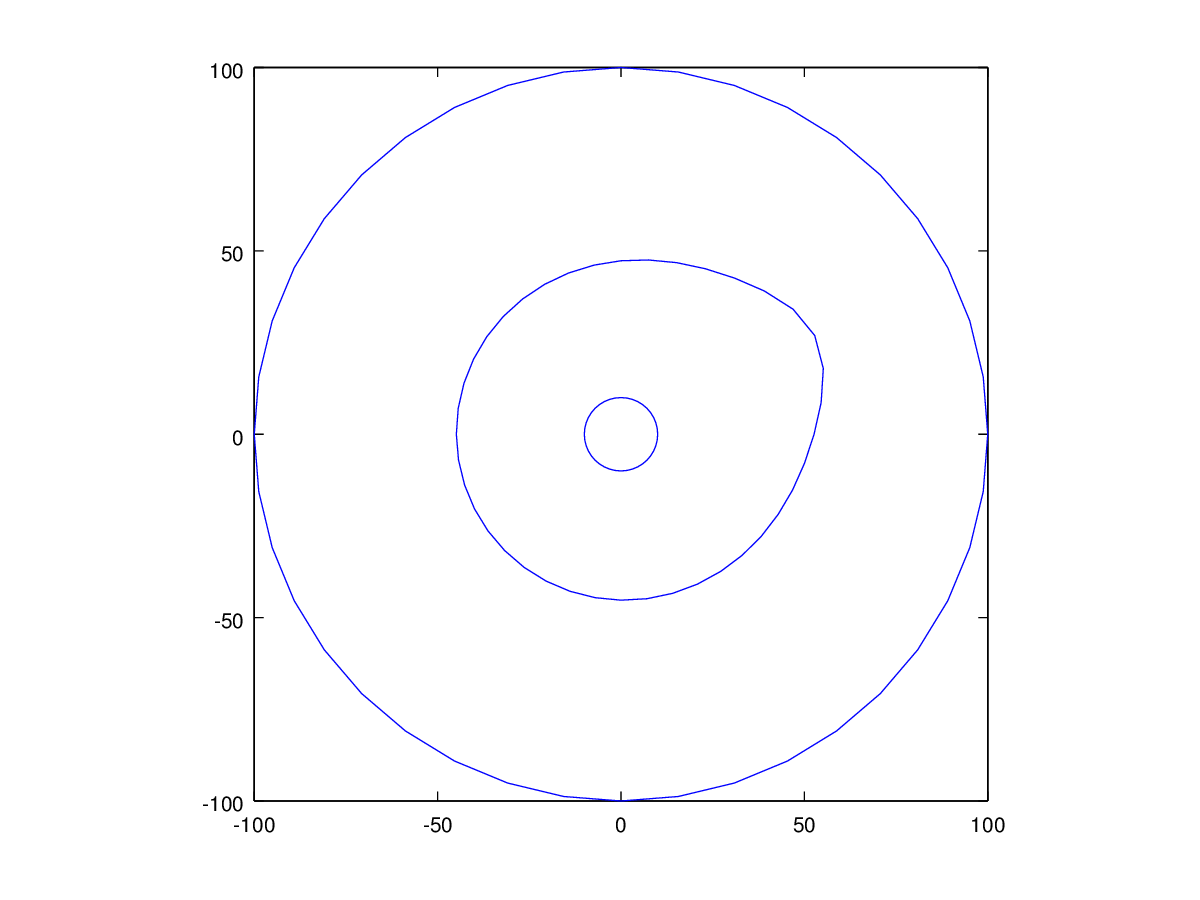
\includegraphics[width=1\textwidth]{imgs/comp_angulos/comp_angs_iso0.png}
  \caption{\footnotesize{Con 300 ángulos se puede detectar a la perfección un pico en la isoterma.}}
  \label{fig:Experimento1}
\end{minipage}%
\hspace{0.03\textwidth}
\begin{minipage}{0.48\textwidth}   
  \centering
    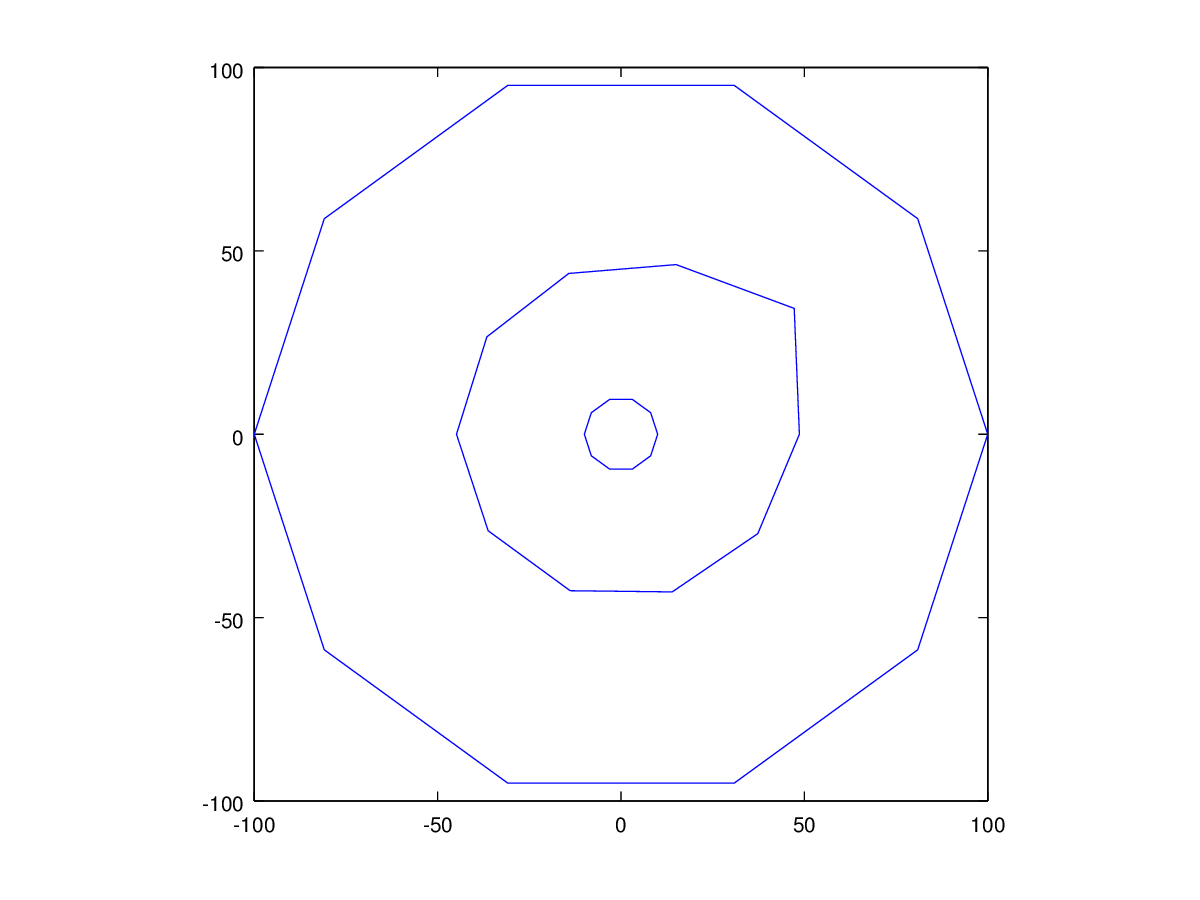
\includegraphics[width=1\textwidth]{imgs/comp_angulos/comp_angs_iso3.png} 
  \caption{\footnotesize{Con 10 ángulos si bien se detecta un pico, la forma que se muestra está muy alejada de la real, esto podría causar falsas alarmas o la ausencia de las mismas.}}
  \label{fig:Experimento2}
\end{minipage}
\end{figure}


\begin{figure}[H]
\begin{minipage}{0.48\textwidth}   
  \centering
    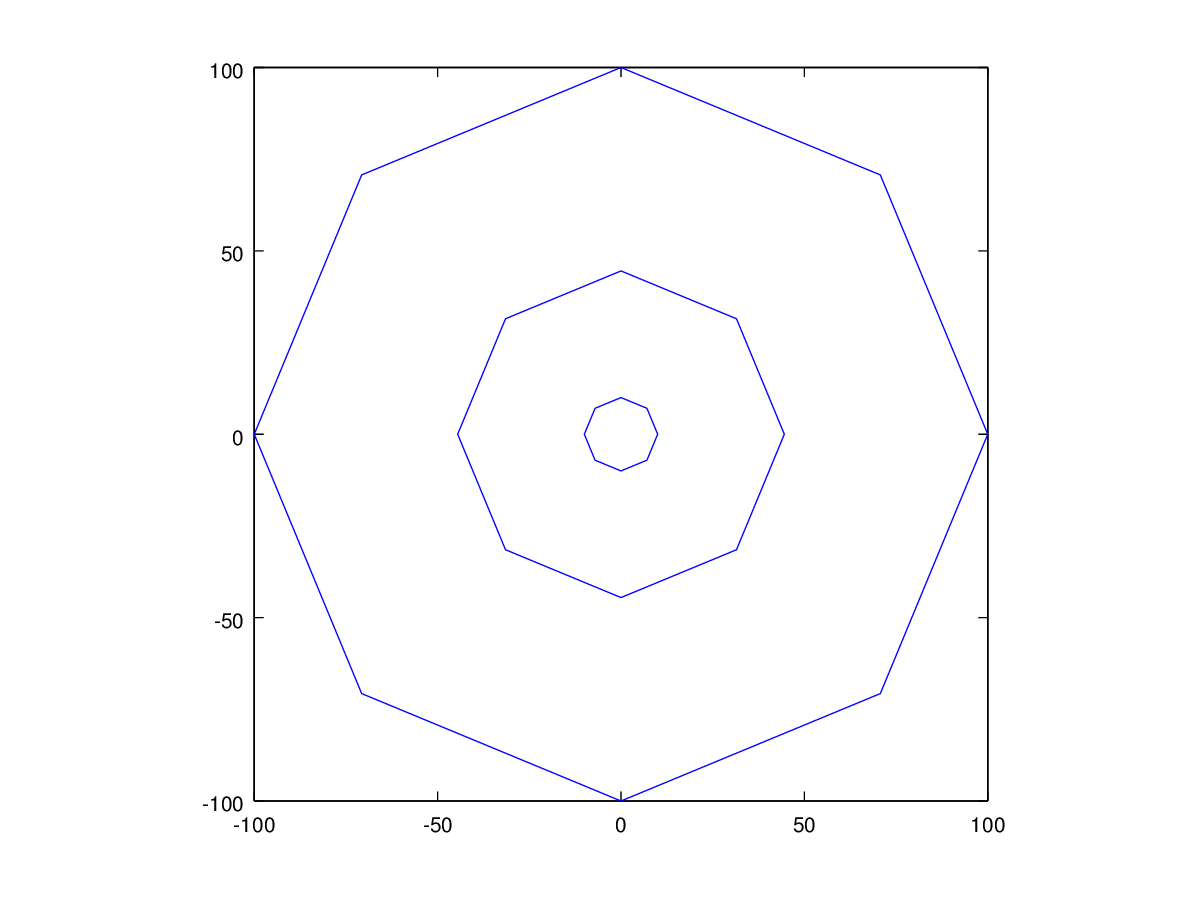
\includegraphics[width=1\textwidth]{imgs/comp_angulos/comp_angs_iso4.png} 
  \caption{\footnotesize{Con 8 ángulos se puede observar como el pico desaparece fallando dramaticamente la predicción en la forma de la isoterma}}
  \label{fig:Experimento3}
\end{minipage}
\end{figure}

\subsubsection{Granularidad de los radios}
Al estudiar las posibilidades en la cantidad de radios a utilizar se puede observar como a mayor granularidad mejora la posición de la isoterma, convergiendo a la posición real. A diferencia de los ángulos, con los radios los picos serán detectados sin tomar demasiadas precauciones pero para asegurar que el tamaño de los picos, y de la isoterma en general, sean predichos de forma confiable se recomendara utilizar una cantidad de radios adecuadamente alta según la necesidad que se tenga.

Para verificar un poco esto utilizamos dos instancias de prueba. La primera forma una isoterma con forma de óvalo debido a un aumento en la temperatura externa en dos zonas opuestas. La segunda es un círculo perfecto producido por una temperatura constante a lo largo de todo el interior y exterior del horno. En ambos casos veremos como la figura va cambiando su tamaño al tender a la isoterma real.

\subsubsection{Instancia 1}

\begin{figure}[H]
\centering
\begin{minipage}{0.48\textwidth}
  \centering
    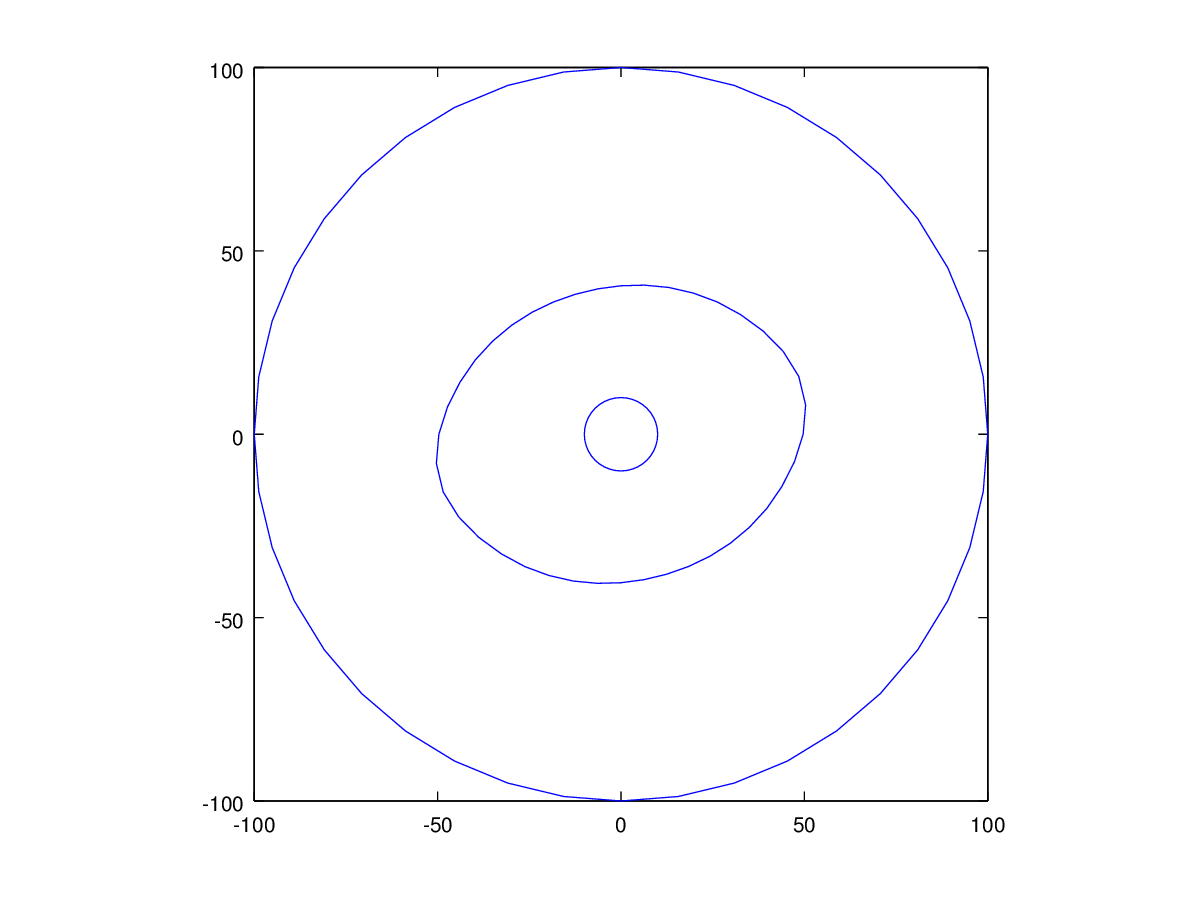
\includegraphics[width=1\textwidth]{imgs/comp_rads_bueno/comp_radss_iso5.png}
  \caption{\footnotesize{Con 30 radios consigue una aproximación muy buena del tamaño de la isoterma.}}
  \label{fig:Radios1}
\end{minipage}%
\hspace{0.03\textwidth}
\begin{minipage}{0.48\textwidth}   
  \centering
    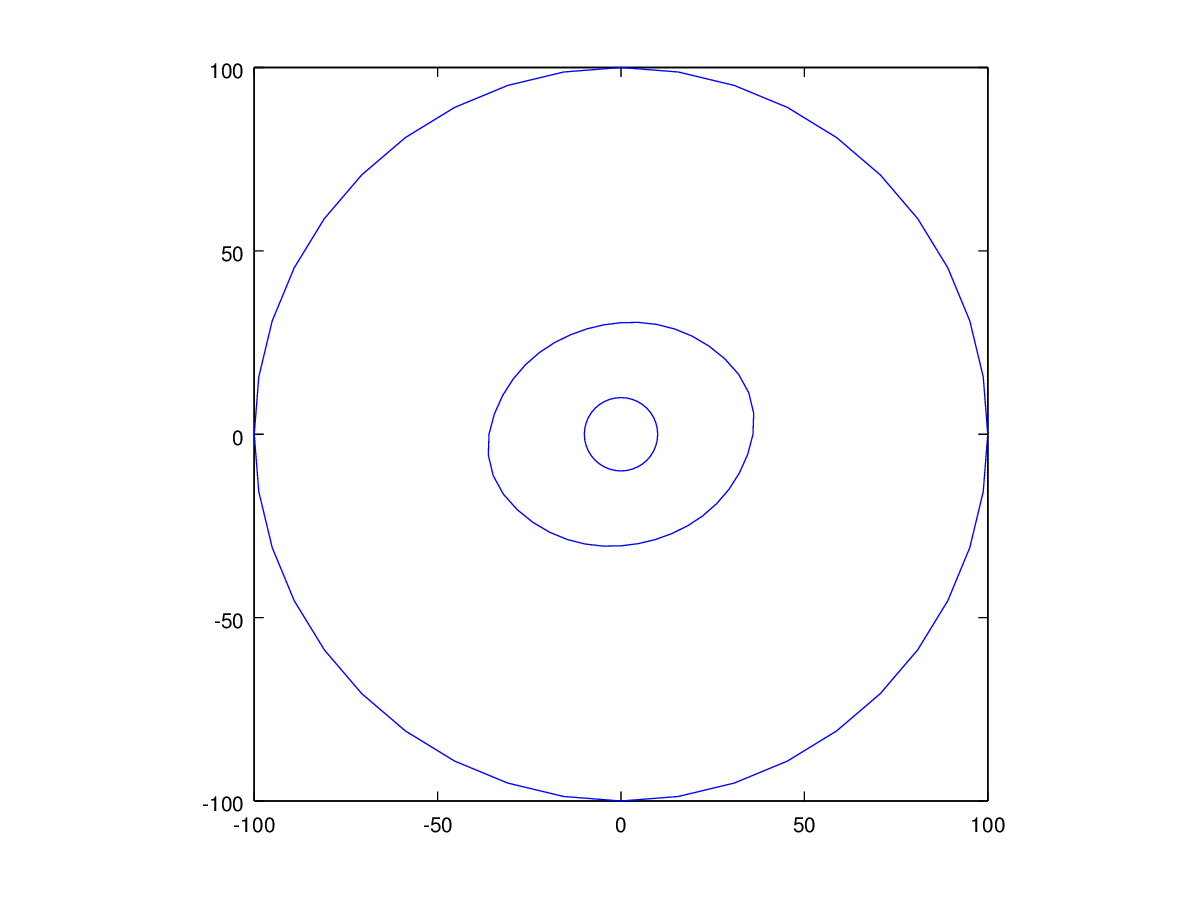
\includegraphics[width=1\textwidth]{imgs/comp_rads_bueno/comp_radss_iso0.png} 
  \caption{\footnotesize{Con 4 radios el tamaño de la isoterma esta muy alejado del real.}}
  \label{fig:Radios2}
\end{minipage}
\end{figure}

\subsubsection{Instancia 2}

  \footnotesize{Sucede lo mismo que en en el experimento anterior, al tomar una cantidad relativamente alta de radios se logra un error muy pequeño del tamaño de la isoterma, en este caso se utilizaron 60. La diferencia entre utilizar 40, 50 y 60 radios no fue muy grande, al menos para nuestros estandares, por lo cual se podrian utilizar simplemente 40 consiguiendo un buena relacion entre tiempo de cálculo y aproximación al tamaño de la isoterma, para apreciar mejor esto pueden acceder a http://bit.ly/1Uqt90x donde alojamos algunas animaciones de nuestros experimentos.}

\begin{figure}[H]
\centering
\begin{minipage}{0.48\textwidth}
  \centering
    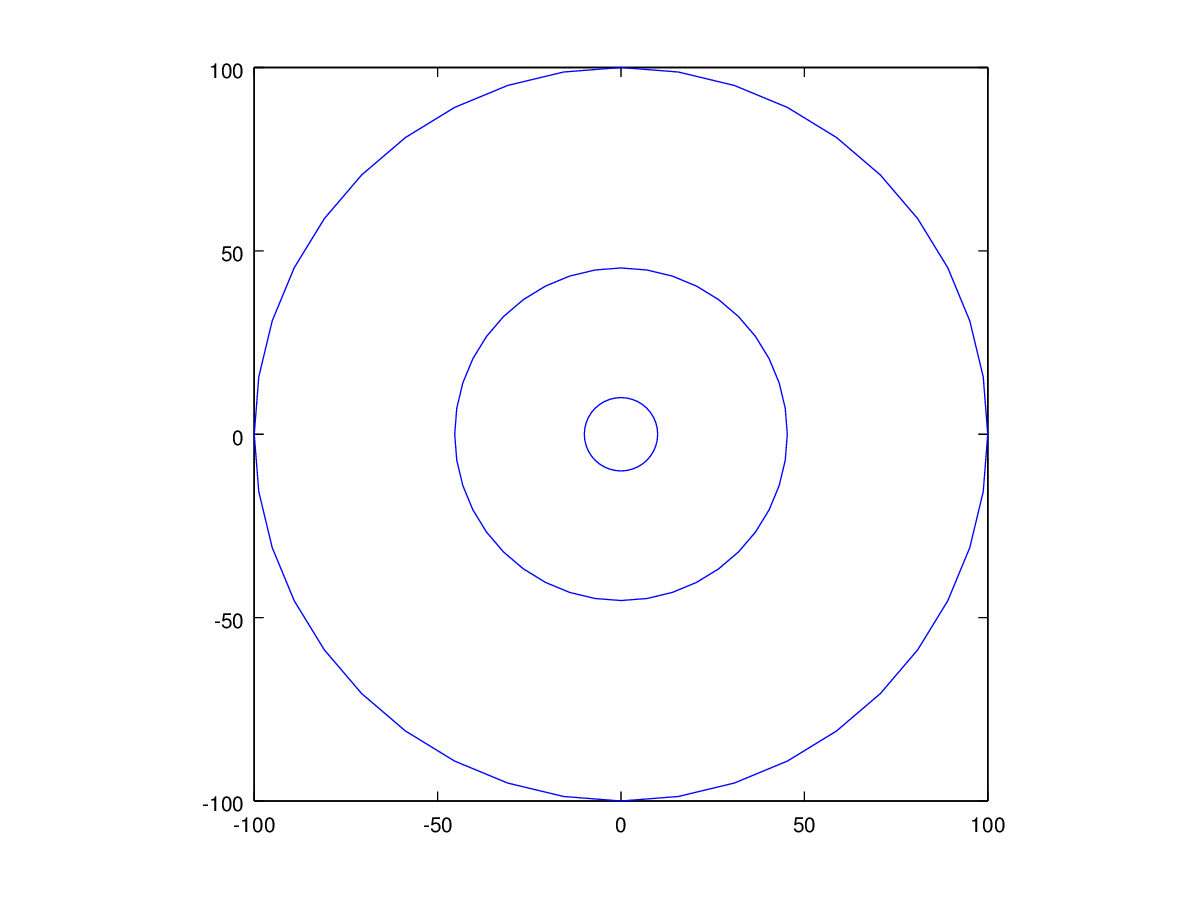
\includegraphics[width=1\textwidth]{imgs/comp_rads_malo/comp_rads_iso5.png}
	\caption{Se utilizaron 60 radios}  
  \label{fig:Radios3}
\end{minipage}%
\hspace{0.03\textwidth}
\begin{minipage}{0.48\textwidth}   
  \centering
    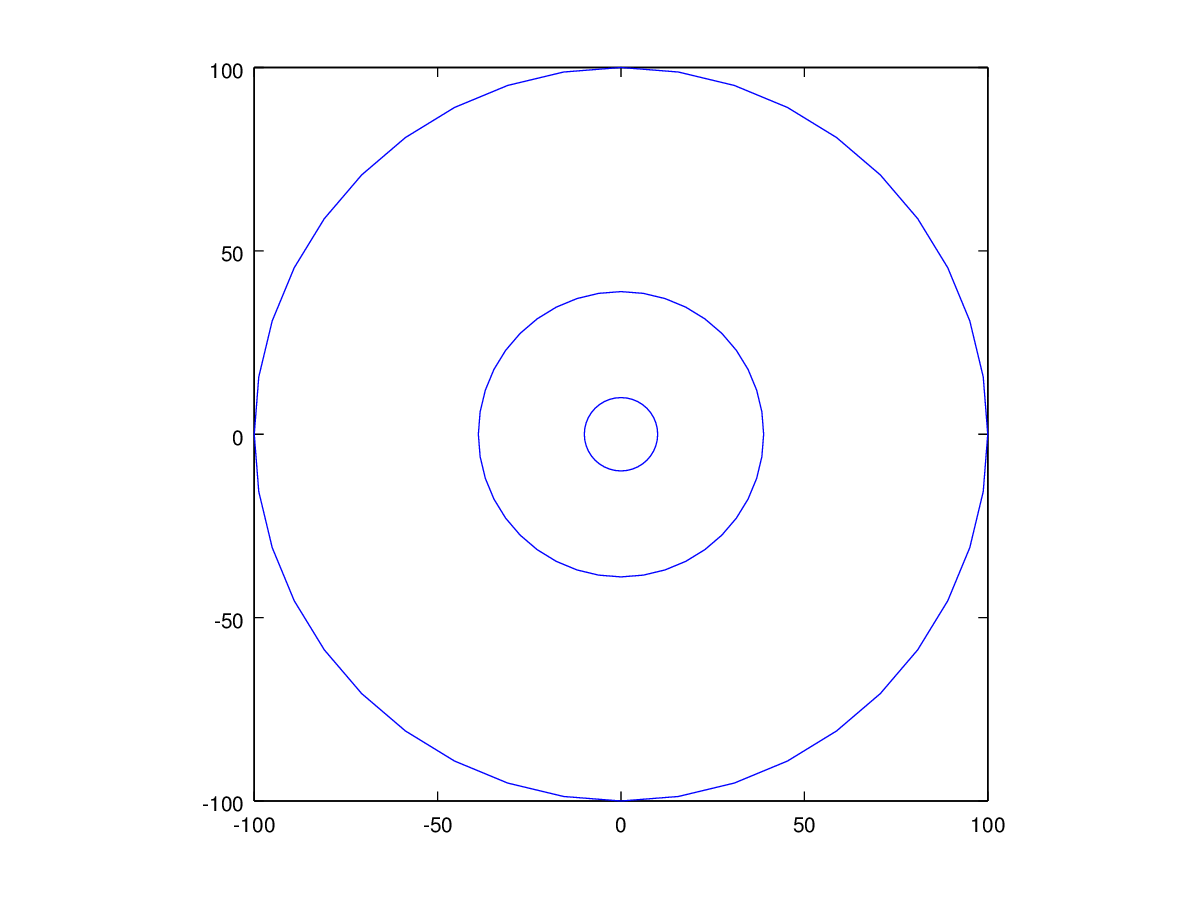
\includegraphics[width=1\textwidth]{imgs/comp_rads_malo/comp_rads_iso0.png} 
	\caption{Se utilizaron 9 radios} 
  \label{fig:Radios4}
\end{minipage}
\end{figure}
